\documentclass{ximera}

\newcommand{\RR}{\mathbb R}
\renewcommand{\d}{\,d}
\newcommand{\dd}[2][]{\frac{d #1}{d #2}}
\renewcommand{\l}{\ell}
\newcommand{\ddx}{\frac{d}{dx}}
\newcommand{\dfn}{\textbf}
\newcommand{\eval}[1]{\bigg[ #1 \bigg]}


\author{Bart Snapp}

\outcome{Undestand the relationship between grad, curl, and div.}

\title[Dig-In:]{Grad, Curl, Div}

\begin{document}
\begin{abstract}
  We explore the relationship between the gradient, the curl, and the
  divergence of a vector field.
\end{abstract}
\maketitle

At this point in our study, we have many fundamental theorems. Let's
try to use them together, and see what we can discover.

\section{A two-dimensional dream}

So far we have two fundamental theorems of calculus for functions of
two variables.
\begin{itemize}
\item The fundamental theorem of line integrals:
  \begin{image}
    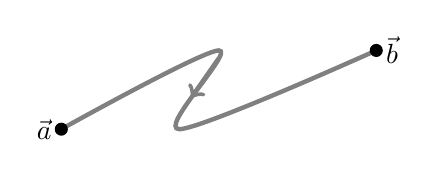
\begin{tikzpicture}
      \draw [ultra thick, gray] plot [smooth] coordinates {(-2,2) (0,3) (-.5,2) (2,3)};
      \draw [ultra thick, gray,->,opacity=1] plot [smooth] coordinates {(0,2.9) (-.35,2.4)};
      214
      \draw[black,fill=black] (-2,2) circle (.5ex);
      \draw[black,fill=black] (2,3) circle (.5ex);
      \node[black,left] at (-2,2) {$\vec{a}$};
      \node[black,right] at (2,3) {$\vec{b}$};
    \end{tikzpicture}
\end{image}
  \[
  \int_C \grad F \dotp\d\vec{p} = F(\vec{b}) -F(\vec{a})
  \]
\item Green's theorem:
  \begin{image}
    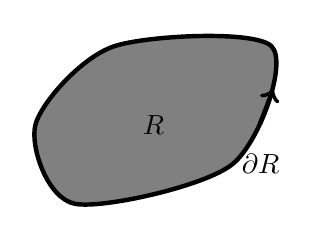
\begin{tikzpicture}
      \draw[ultra thick, black,fill=gray] plot [smooth cycle] coordinates {(-1.5,.5) (.5,1) (1,2.5) (-1,2.5) (-2,1.5)};
      \draw[ultra thick,black, ->] plot [smooth] coordinates {(.85,1.51) (1.02,1.95)};
      \node[black] at (-.5,1.5) {$R$};
      \node[black,right] at (.5,1) {$\partial R$};
    \end{tikzpicture}
  \end{image}
  \[
  \iint_R \curl \vec{F} \d A = \oint_{\partial R} \vec{F} \dotp \d \vec{p}
  \]
\end{itemize}
Wouldn't it be cool if we could \textit{combine} these theorems to
make something like:
\[
\iint_R \curl \grad F \d A = \oint_{\partial R} \grad F \dotp \d \vec{p} = F(\vec{b}) - F(\vec{a})
\]
A double integral, equaling a single integral, equaling a difference!
It's an amazing idea, and while it is true, we shouldn't get too
excited. In fact each expression above is equal to zero. Let's see
why.

First note that both sides of the equation:
\[
\oint_{\partial R} \grad F \dotp \d \vec{p} = F(\vec{b}) - F(\vec{a})
\]
are zero. This is because, with a closed curve, $\vec{a}=\vec{b}$, and
so $F(\vec{a}) = F(\vec{b})$. But this means that
\[
\iint_R \curl \grad F \d A = 0
\]
Note, this is totally independent of the region $R$ and
the surface $F$. The upshot: $\curl\grad F = 0$ for all functions
$\vec{F}:\R^2\to\R^2$ with continuous second derivatives!

\begin{question}
  Let $F:\R^2\to \R$ be a function with continuous second
  derivatives. Which of the following make sense?
  \begin{selectAll}
    \choice[correct]{$\grad F$}
    \choice{$\curl F$}
    \choice{$\divergence F$}
    \choice[correct]{$\curl\grad F$}
    \choice{$\curl \divergence F$}
    \choice[correct]{$\divergence \grad F$}
    \choice{$\divergence \curl F$}
  \end{selectAll}
  \begin{question}
    Of the choices above that make sense, which must be equal to $0$?
    \begin{prompt}
    \begin{selectAll}
      \choice{$\grad F$}
      \choice[correct]{$\curl\grad F$}
      \choice{$\divergence \grad F$}
    \end{selectAll}
    \end{prompt}
    \end{question}
\end{question}

Of course, you could poo-poo the work above and say ``I already knew
that!  This is just the Clairaut gradient test!'' Well, sure, but
what we just presented is \textit{another} reason that $\curl \grad F
= 0$. Moreover, this line of reasoning will lead us to new ideas
too. Read-on young mathematician, there is not much further to go in
this course.



\section{A three-dimensional dream}

Working in a similar way to how we worked above, let us recall the fundamental theorems of calculus for functions of three variables.

\begin{itemize}
\item The fundamental theorem of line integrals:
  \begin{image}
    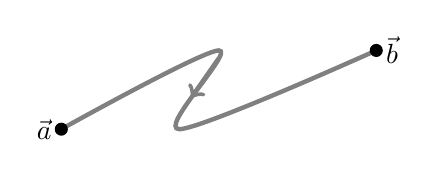
\begin{tikzpicture}
      \draw [ultra thick, gray] plot [smooth] coordinates {(-2,2) (0,3) (-.5,2) (2,3)};
      \draw [ultra thick, gray,->,opacity=1] plot [smooth] coordinates {(0,2.9) (-.35,2.4)};
      \draw[black,fill=black] (-2,2) circle (.5ex);
      \draw[black,fill=black] (2,3) circle (.5ex);
      \node[black,left] at (-2,2) {$\vec{a}$};
      \node[black,right] at (2,3) {$\vec{b}$};
    \end{tikzpicture}
\end{image}
  \[
  \int_C \grad F \dotp\d\vec{p} = F(\vec{b}) - F(\vec{a}) 
  \]
\item Stokes' Theorem:
  \begin{image}
    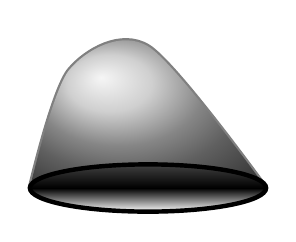
\begin{tikzpicture}
      \draw[gray,ultra thick] plot[smooth] coordinates {(-1.5,1.5) (-1,3) (0,3.3)  (1.5,1.5)};
      \shade[ball color=white!50!gray] plot[smooth] coordinates {(-1.5,1.5) (-1,3) (0,3.3)  (1.5,1.5)};
      \shade[top color=black!50!gray, middle color=black]  (0,1.5) ellipse (1.5 and .3);
      \draw[black,ultra thick] (0,1.5) ellipse (1.5 and .3);
    \end{tikzpicture}
  \end{image}
  \[
  \iint_R \curl\vec{F}\dotp \uvec{n} \d S = \oint_{\partial R} \vec{F} \dotp \d \vec{p}
  \]
\item The Divergence Theorem:
  \begin{image}
  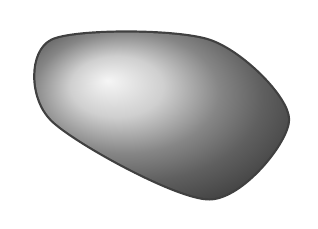
\begin{tikzpicture}
    \draw[ultra thick, gray!50!black] plot [smooth cycle] coordinates {(-1.5,2) (.5,1) (1.5,2) (.5,3) (-1.5,3)};
    \shade[ball color=gray!50!white] plot [smooth cycle] coordinates {(-1.5,2) (.5,1) (1.5,2) (.5,3) (-1.5,3)};
  \end{tikzpicture}
\end{image}

  \[
  \iiint_R \divergence\vec{F} \d V = \oiint_{\partial R} \vec{F}\dotp\uvec{n} \d S
  \]
\end{itemize}
Putting Stokes' Theorem and the Divergence Theorem together, we find the beautiful expression:
\[
\iiint_R \divergence\left(\curl\vec{F}\right)\d V = \oiint_{\partial R} \left(\curl \vec{F}\right)\dotp \uvec{n} \d S = \oint_{\partial\partial R} \vec{F}\dotp \d \vec{p}
\]
Again, what a fantastic idea, a triple integral, equaling a double
integral, equaling a single integral! However, there is again a rub,
the boundary of a closed curve is \textit{empty}. A closed curve has
\textbf{no boundary}! Hence:
\[
\oint_{\partial\partial R} \vec{F}\dotp \d \vec{p} = 0
\]
This fact, in turn means that all of the integrals above, including:
\[
\iiint_R \divergence\left(\curl\vec{F}\right)\d V = \oiint_{\partial R} \left(\curl \vec{F}\right)\dotp \uvec{n} \d S
\]
Are all equal to to zero!  We thus conclude:
\begin{itemize}
\item $\oiint_{\partial R} \left(\curl \vec{F}\right)\dotp \uvec{n} \d
  S=0$ tells us that the circulation along \textbf{any} closed surface
  is zero, and
\item $\iiint_R \divergence\left(\curl\vec{F}\right)\d V = 0$ tells us
  that for any vector field $\vec{F}:\R^3\to\R^3$,
  $\divergence\left(\curl\vec{F}\right)=0$.
\end{itemize}

Let's see what you can do now.


\begin{question}
  Let $F:\R^3\to \R$ be a function with continuous second derivatives
  and let $\vec{G}:\R^3\to\R^3$ be a vector field. Which of the
  following make sense?
  \begin{selectAll}
    \choice{$\curl F$}
    \choice[correct]{$\curl \vec{G}$}
    \choice{$\divergence F$}
    \choice[correct]{$\curl\grad F$}
    \choice{$\curl \divergence F$}
    \choice{$\curl \divergence \vec{G}$}
    \choice[correct]{$\divergence \grad F$}
    \choice[correct]{$\divergence\left(\curl \vec{G}\right)$}
  \end{selectAll}
  \begin{question}
    Of the choices above that make sense, which must be equal to $0$
    or $\vec{0}$?
    \begin{prompt}
      \begin{selectAll}
        \choice{$\curl \vec{G}$}
        \choice[correct]{$\curl\grad F$}
        \choice{$\divergence \grad F$}
        \choice[correct]{$\divergence\left(\curl \vec{G}\right)$}
    \end{selectAll}
    \end{prompt}
    \end{question}
\end{question}



\section{The shape of things to come}

Recalling that $C^\infty(A,B)$ is the set of differentiable functions
from $A$ to $B$ where \textbf{all} of the derivatives are continuous,
we can make the following ``chain'' of derivatives:
\begin{image}
  \begin{tikzpicture}
    \node{
    \begin{tikzcd}[ampersand replacement=\&,row sep=-.5em]
     C^{\infty}(\R^2,\R) \arrow[r,"\grad"] \& C^{\infty}(\R^2,\R^2) \arrow[r,"\curl"] \& C^{\infty}(\R^2,\R)\\
     F \arrow[r,mapsto] \& \grad F  \arrow[r,mapsto] \& 0
    \end{tikzcd}};
  \end{tikzpicture}
\end{image}
From our work above (and from previous parts of this course) we will
always have that $\curl\grad F = 0$.


Since the Fundamental Theorem of Line Integrals (FTLI) is in some
sense about ``undoing'' the gradient and Green's Theorem is in some
sense about ``undoing'' the scalar curl, we can also place these in
the diagram:
\begin{image}
  \begin{tikzpicture}
    \node{
    \begin{tikzcd}[ampersand replacement=\&,row sep=-.5em]
     C^{\infty}(\R^2,\R) \arrow[r,"\grad"] \& \arrow[l,"\text{FTLI}",bend left=20 ]C^{\infty}(\R^2,\R^2) \arrow[r,"\curl"] \& \arrow[l,"\text{Green's Theorem}", bend left =20]C^{\infty}(\R^2,\R)
    \end{tikzcd}};
  \end{tikzpicture}
\end{image}

Working in a similar way, we can make a chain of derivatives in three-dimensions as well:
\begin{image}
  \begin{tikzpicture}
    \node{
  \begin{tikzcd}[ampersand replacement=\&, row sep=-.5em,column sep=4ex]
    C^{\infty}(\R^3,\R) \arrow[r,"\grad"] \& C^{\infty}(\R^3,\R^3) \arrow[r,"\curl"] \& C^{\infty}(\R^3,\R^3) \arrow[r,"\divergence"] \& C^{\infty}(\R^3,\R)\\
    F \arrow[r,mapsto] \& \grad F  \arrow[r,mapsto] \& \vec{0}   \&\\
                       \& \vec{G}  \arrow[r,mapsto] \& \curl\vec{G} \arrow[r,mapsto]   \& 0
    \end{tikzcd}};
  \end{tikzpicture}
\end{image}
From our work above, we always will have that $\curl\grad F = \vec{0}$
and $\divergence\left(\curl \vec{G}\right) = 0$.

Since Stokes' Theorem is in some sense about ``undoing'' the curl and
the Divergence Theorem is in some sense about ``undoing'' the
divergence, we can place these theorems into the diagram as well:
\begin{image}
  \begin{tikzpicture}
    \node{
  \begin{tikzcd}[ampersand replacement=\&, row sep=-.5em,column sep=4ex]
    C^{\infty}(\R^3,\R) \arrow[r,"\grad"] \& \arrow[l,"\text{FTLI}",bend left = 20]C^{\infty}(\R^3,\R^3) \arrow[r,"\curl"] \& \arrow[l,"\text{Stokes' Theorem}",bend left = 20] C^{\infty}(\R^3,\R^3) \arrow[r,"\divergence"] \&  \arrow[l,"\text{Divergence Theorem}",bend left = 20]C^{\infty}(\R^3,\R)
    \end{tikzcd}};
  \end{tikzpicture}
\end{image}

Now let's get crazy. Let's put all of our diagrams together into one big diagram: 
\begin{image}
  \begin{tikzpicture}
    \node{
      \begin{tikzcd}[ampersand replacement=\&, row sep=tiny, column sep=-5ex]
        \& \& C^{\infty}(\R,\R) \arrow[rr,"\ddx"] \& \& C^{\infty}(\R,\R) \& \& \\
        \& C^{\infty}(\R^2,\R) \arrow[rr,"\grad"] \& \& C^{\infty}(\R^2,\R^2) \arrow[rr,"\curl"] \& \& C^{\infty}(\R^2,\R) \&\\
        C^{\infty}(\R^3,\R) \arrow[rr,"\grad"] \& \& C^{\infty}(\R^3,\R^3) \arrow[rr,"\curl"] \& \& C^{\infty}(\R^3,\R^3) \arrow[rr,"\divergence"] \& \& C^{\infty}(\R^3,\R)
    \end{tikzcd}};
  \end{tikzpicture}
\end{image}

Checkout the values for $n$ in each of the $C^\infty(\R^m,\R^n)$:

\begin{image}
  \begin{tikzpicture}
    \node{
      \begin{tikzcd}[ampersand replacement=\&, row sep=tiny, column sep=-5ex]
        \& \& C^{\infty}(\R,\R^{\mathbf{1}}) \arrow[rr,"\ddx"] \& \& C^{\infty}(\R,\R^{\mathbf{1}}) \& \& \\
        \& C^{\infty}(\R^2,\R^{\mathbf{1}}) \arrow[rr,"\grad"] \& \& C^{\infty}(\R^2,\R^{\mathbf{2}}) \arrow[rr,"\curl"] \& \& C^{\infty}(\R^2,\R^{\mathbf{1}}) \&\\
        C^{\infty}(\R^3,\R^{\mathbf{1}}) \arrow[rr,"\grad"] \& \& C^{\infty}(\R^3,\R^{\mathbf{3}}) \arrow[rr,"\curl"] \& \& C^{\infty}(\R^3,\R^{\mathbf{3}}) \arrow[rr,"\divergence"] \& \& C^{\infty}(\R^3,\R^{\mathbf{1}})
    \end{tikzcd}};
  \end{tikzpicture}
\end{image}
Here they are by themselves:
\[
\begin{array}{ccccccc}
    &   & 1 &   & 1 &   &   \\
    & 1 &   & 2 &   & 1 &   \\
  1 &   & 3 &   & 3 &   & 1
\end{array}
\]
These are rows of \link[Pascal's
  Triangle]{https://en.wikipedia.org/wiki/Pascal_triangle}! For each
row we find more fundamental theorems of calculus. Moreover, the
triangle can be extended, for example:
\begin{image}
  \begin{tikzpicture}
    \node{
      \begin{tikzcd}[ampersand replacement=\&, row sep=tiny, column sep=-5ex]
        \& \& \& C^{\infty}(\R,\R^{{1}}) \arrow[rr,"\ddx"] \& \& C^{\infty}(\R,\R^{{1}}) \& \& \&  \\
        \& \& C^{\infty}(\R^2,\R^{{1}}) \arrow[rr,"\grad"] \& \& C^{\infty}(\R^2,\R^{{2}}) \arrow[rr,"\curl"] \& \& C^{\infty}(\R^2,\R^{{1}}) \& \&\\
        \& C^{\infty}(\R^3,\R^{{1}}) \arrow[rr,"\grad"] \& \& C^{\infty}(\R^3,\R^{{3}}) \arrow[rr,"\curl"] \& \& C^{\infty}(\R^3,\R^{{3}}) \arrow[rr,"\divergence"] \& \& C^{\infty}(\R^3,\R^{{1}}) \& \\
        C^\infty(\R^4,\R^1) \arrow[rr] \&  \& C^\infty(\R^4,\R^4) \arrow[rr] \&  \& C^\infty(\R^4,\R^6) \arrow[rr] \&  \& C^\infty(\R^4,\R^4) \arrow[rr] \&  \& C^\infty(\R^4,\R^1) 
    \end{tikzcd}};
  \end{tikzpicture}
\end{image}
In the fourth row, there are four(!) fundamental theorems of calculus. Moreover, this triangle can be extended \textit{infinitely!} The details of this are beyond the scope of this course. Math folks who know this eventually start calling all of these fundamental theorems ``\link[Stokes' Theorem]{https://en.wikipedia.org/wiki/Stokes_theorem}.''

Alas, our course has come to an end. However, it is really much more of a \textbf{beginning,} as there is \textbf{so much more to know.} 

\end{document}
